\documentclass{article}
\usepackage{arxiv}
%\documentclass[12pt]{article}
%\usepackage[cp1251]{inputenc}
%\usepackage[russian]{babel}

\usepackage[utf8]{inputenc}
\usepackage[english, russian]{babel}
\usepackage[T2A, T1]{fontenc}
\usepackage{url}
\usepackage{booktabs}
\usepackage{amsfonts}
\usepackage{nicefrac}
\usepackage{microtype}
\usepackage{lipsum}
\usepackage{comment}
\usepackage{graphicx}
\usepackage{natbib}
\usepackage{doi}
\usepackage{hyperref}
\usepackage{amssymb, amsmath, latexsym}
% \usepackage{fullpage}
\usepackage{algorithm}
\usepackage{algorithmic}
%\usepackage{algpseudocode}
\usepackage{tabularx}
\usepackage{paralist}
\usepackage{mathtools}
%\usepackage{tcolorbox}
\usepackage{xcolor}
\usepackage{amsmath}
\DeclareMathOperator*{\argmax}{arg\,max}
\DeclareMathOperator*{\argmin}{arg\,min}

\usepackage{bbm} %for indicators 1

\usepackage{makecell}
\usepackage{multirow}
\usepackage{booktabs}
\usepackage{caption}
\usepackage{subcaption}

\usepackage{nicefrac}  
\usepackage{hyperref}
\usepackage{subcaption}
% \usepackage{subfigure} 
\newcommand{\Exp}{\mathbf{E}}
\newcommand{\Prob}{\mathbf{P}}
\newcommand{\R}{\mathbb{R}}
\newcommand{\eqdef}{\stackrel{\text{def}}{=}}


\newtheorem{Def}{Определение}[section]
\newtheorem{proposition}{Предположение}

\title{Жадный метод оптимизации первого порядка с относительным шумом}

\author{
	Рубцов Денис \\
	\texttt{rubtsov.dn@phystech.edu} \\
	%% examples of more authors
	\And
	Корнилов Никита \\
	\texttt{kornilov.nm@phystech.edu} \\
	%% \AND
	%% Coauthor \\
	%% Affiliation \\
	%% Address \\
	%% \texttt{email} \\
	%% \And
	%% Coauthor \\
	%% Affiliation \\
	%% Address \\
	%% \texttt{email} \\
	%% \And
	%% Coauthor \\
	%% Affiliation \\
	%% Address \\
	%% \texttt{email} \\
}
\date{}

\renewcommand{\shorttitle}{Жадный метод оптимизации первого порядка с относительным шумом}
\renewcommand{\undertitle}{}
%%% Add PDF metadata to help others organize their library
%%% Once the PDF is generated, you can check the metadata with
%%% $ pdfinfo template.pdf
\hypersetup{
pdftitle={Жадный методы оптимизации первого порядка с относительным шумом},
pdfsubject={Методы оптимизации первого порядка},
pdfauthor={Рубцов Д.Н., Корнилов Н.М.},
pdfkeywords={методы оптимизации первого порядка, жадные методы, неточный градиент, относительный шум, Performance Estimation Problem, машинное обучение},
}

\begin{document}
\maketitle

\begin{abstract}
Работа посвящена жадному методу гладкой выпуклой оптимизации первого порядка с градиентами, известными лишь с некоторой относительной погрешностью. С помощью численной техники PEP получена эмпирическая гипотеза о влиянии этой погрешности на скорость сходимости метода. 

\end{abstract}


\keywords{: методы оптимизации первого порядка, жадные методы, неточный градиент, относительный шум, Performance Estimation Problem, машинное обучение}

\section{Введение}

В данной статье изучаются методы гладкой выпуклой оптимизации первого порядка. Их изучение актуально в связи с высоким успехом их применения во многих приложениях, в том числе в машинном обучении (см., например, в \cite{bottou2007tradeoffs}). Эти методы (например, Adam (\cite{kingma2014adam})) позволяют эффективно решать задачи многомерной оптимизации, в том числе и невыпуклой.

Во многих ситуациях алгоритмы не имеют доступа к точному градиенту. Так, например, бывает, когда для того, чтобы получить значение градиента, требуется решить другую сложную задачу (например, решить дифференциальное уравнение, см. в \cite{matyukhin2021convex}). В данной статье мы сосредоточимся на случае, когда градиенты известны с некоторой относительной погрешностью $\varepsilon \in [0, 1]$: $$\|\widetilde{\nabla} f(x) - \nabla f(x)\|_2 \leq \varepsilon \|\nabla f(x)\|_2.$$
Часто доказательства скорости сходимости методов оптимизации носят неинтуитивный, техничный характер. Они представляют собой цепочку длинных нетривиальных неравенств, оценивающих наихудший случай. Численное решение задачи поиска наихудшего случая может быть осуществлено с помощью техники Performance Estimation Problem (далее -- PEP, см. в \cite{goujaud2022pepit}, \cite{taylor2017smooth}, \cite{taylor2017convex}), которая применяется с этой целью и в данной статье.

\subsection{Определения и обозначения}

\begin{comment}
    В таблице 1 приведены некоторые обозначения, используемые в работе 

\begin{table}[h!]\label{def_table}
\caption{Список обозначений, используемых в работе}
\centering
 \begin{tabular}{||p{2 cm} | p{8cm}||} 
 \hline

 $\mathcal{F}_{\mu, L}$ & Класс $\mu$-сильно выпуклых $L$-гладких функций  \\ 
 \hline
 \langle x,y \rangle & Скалярное произведение векторов $x,y \in \R^n$  \\
 \hline
 $\|x\|_2$ & $\ell_2$-норма элемента $x \in \R^n$  \\
 \hline
 $x_0$ & Начальная точка  \\
 \hline
 $k$ & Номер текущей итерации алгоритма  \\
 \hline
 $N$ & Полное число итераций алгоритма \\
 \hline
 $\mathcal{O}^{(f)}$ & Ответ оракула  \\ 
 \hline
 $\mathcal{A}$ & Алгоритм (правило генерации последовательностей $(x_k)_{k \le N}$ приближений точки минимума $x_{\star}$ функции $f$) \\
 \hline
 $(x_k)_{k \le N}$ & Последовательность точек  \\[1ex] 
 \hline
 \end{tabular}
\end{table}
\end{comment}




В данной работе будут решаться задачи оптимизации в следующих предположениях на исследуемые функции $f$.

\begin{proposition}
    Функция $f$ --- $\mu$-сильно выпукла, если существует константа $\mu > 0$ такая, что:
    \begin{equation}\label{eq:str_cvx}
        f(y) \geq f(x) + \langle \nabla f(x), y - x \rangle + \frac{\mu}{2}\|y - x\|_2^2, \quad x, y \in \R^n. 
    \end{equation}
\end{proposition}


\begin{proposition}
    Функция $f$ --- $L$-гладкая, если существует константа $L > 0$ такая, что:
\begin{equation}\label{smoothness_cond}
    f(y) \leq f(x)+ \left\langle\nabla f(x), y-x\right\rangle + \frac{L}{2} \|y-x\|_2^2, \quad \forall x, y \in \mathbb{R}^n,
\end{equation}
или (эквивалентно) 
\begin{equation}\label{eq_6}
    \|\nabla f(y) - \nabla f(x)\|_2 \leq L \|y - x\|_2, \quad \forall x, y \in \mathbb{R}^n.
\end{equation}
\end{proposition}

Множество $\mu$-сильно выпуклых $L$-гладких функций будем обозначать $\mathcal{F}_{\mu, L}$.


\begin{proposition}
    \label{inexact_grad}
Будем говорить, что мы имеем доступ к градиенту функции $f$ с некоторой относительной погрешностью $\varepsilon \in [0, 1]$, если
\begin{equation}\label{eq_relative_error}
    \|\widetilde{\nabla} f(x) - \nabla f(x)\|_2 \leq \varepsilon\|\nabla f(x)\|_2 \ \forall x \in \mathbb{R}^n.
\end{equation}
Здесь $\nabla f(x)$ --- точное значение градиента функции $f$ в точке $x$, а $\widetilde{\nabla} f(x)$ --- доступное нам зашумленное значение градиента.
\end{proposition} 

%\begin{Def}
%Класс всех $L$-гладких, $\mu$-сильно выпуклых функций будем обозначать $\mathcal{F}_{\mu, L}$. Класс всех $L$-гладких, выпуклых функций будем обозначать $\mathcal{F}_{0, L}$
%\end{Def}

\subsection{Жадный метод оптимизации первого порядка (GFOM)}



Классические методы оптимизации первого порядка включают в себя градиентный спуск (GD, \cite{cauchy1847methode}), метод тяжелого шарика Б.Т. Поляка (HB, \cite{polyak1963gradient}) и ускоренный метод Ю.Е. Нестерова (NAG, \cite{nesterov1983method}). Так, итерация метода градиентного спуска записывается в следующем виде:
\[x_{k+1}  = x_k - \alpha \nabla f(x_k). \tag{GD}\]
Итерация метода тяжелого шарика:
\[x_{k+1} = x_k - \alpha \nabla f(x_k) + \beta (x_k - x_{k - 1}).\tag{HB}\]
Итерация ускоренного метода Ю.Е. Нестерова:
\[x_{k+1} = x_k - h \nabla f(x_k + \frac{k - 1}{k + 2} (x_k - x_{k-1})) + \frac{k - 1}{k + 2} (x_k - x_{k-1}).\tag{NAG}\]

В каждом из этих методов результат $k$-ой итерации $x_k$ линейно выражается через результаты предыдущих итераций $(x_s)_{s < k}$ и предыдущие ответы оракула $(\nabla f(x_s))_{s < k}$. В случае методов оптимизации первого порядка ответы оракула --- это градиенты $\nabla f(x)$ или неточные градиенты $\widetilde{\nabla} f(x)$.

Так и жадный метод оптимизации первого порядка (Greedy first-order method GFOM, см. в \cite{drori2020efficient}) результат $k$-ой итерации $x_k$ выражает через начальную точку $x_0$ и линейную комбинацию ($\text{span}$) градиентов на предыдущих шагах $(\nabla f(x_s))_{s < k}$
\[x_k = \argmin_{x \in \mathbb{R}^n}\{f(x): x \in x_0 + \text{span}\{\nabla f(x_0), ..., \nabla f(x_{k-1})\}\}. \tag{GFOM}\]
Таким образом, на каждой итерации GFOM жадно находит оптимальную линейную комбинацию градиентов функции в точках, полученных на предыдущих итерациях. Оптимальность здесь имеется в виду в смысле минимальности значения функции на этой комбинации.  



%\subsection{Performance Estimation Problem (PEP)}

%Особое место в данной статье отведено технике Performance Estimation Problem (далее -- PEP, см. в \cite{goujaud2022pepit}, \cite{taylor2017smooth}, \cite{taylor2017convex}). С помощью этого инструмента исследования в данной статье демонстрируется точность полученной ранее в статье \cite{kornilov2023intermediate} теоретической оценки максимальной погрешности, сохраняющей сходимость метода ISTM. Более того, с помощью этой техники проводится поиск оптимальных методов первого порядка, основанных на принципе жадных алгоритмов (\cite{goujaud2023fundamental}, \cite{kim2018generalizing}). 



%\subsection{Intermediate Similar Triangle Method with Relative Noise in Gradient}

%В статье \cite{kornilov2023intermediate} рассматривается алгоритм Intermediate Similar Triangle Method. В этой работе была получена наилучшая из известных на данный момент оценок максимальной относительной погрешности, сохраняющей сходимость этого метода в случае сильной выпуклости $\hat{\varepsilon} \lesssim (\mu / L)^{1/2}$. Более того, в выпуклом случае было показано, что при малом числе итераций $N$ алгоритм сходится со скоростью $\sim \frac{1}{N^p}$. Однако при числе итераций $N: N^p \hat{\varepsilon}^2 \gtrsim 1$, близость к оптимальному значению функции выходит на плато $\hat{\varepsilon}^2 L R_0^2$, где $R_0 = \|x^0 - x^*\|_2$, а $L$ --- константа гладкости.  Эти оценки были подтверждены с помощью численных экспериментов, использующих технику PEP, в той же статье. В нашей статье проводятся дополнительные численные эксперименты.

\begin{comment}
\begin{algorithm}[!ht]
caption{ Intermediate  Similar Triangle Method (\texttt{ISTM}).}\label{alg_STM_relative}
\begin{algorithmic}[1]
   \REQUIRE Initial point $x^0$, number of iterations $N$, smoothness constant  $L>0$, and step size parameter $a \geq 1$, intermediate parameter $p \in [1,2]$. 
   \STATE Set $A_0 = \alpha_0 = 0, y^0 = z^0 = x^0$.
   \FOR{$k=0,1 ,  \ldots, N-1$}
   \STATE Set $\alpha_{k+1} = \frac{(k+2)^{p-1}}{2aL}, \, A_{k+1} = \alpha_{k+1} + A_k$. \label{item_3}
   \STATE $x^{k+1} = \frac{1}{A_{k+1}} \left(A_k y^k + \alpha_{k+1} z^k\right) $. \label{item_4}
   \STATE $z^{k+1} = z^k - \alpha_{k+1} \widetilde{\nabla} f(x^{k+1})$.
   \STATE $y^{k+1} = \frac{1}{A_{k+1}} \left(A_k y^k + \alpha_{k+1} z^{k+1}\right)$.
   \ENDFOR
    \ENSURE 
	$y^N$.
\end{algorithmic}
\end{algorithm}
\end{comment}

%\subsection{О поиске оптимальных методов}
%Во всех статьях (в том числе, в \cite{kornilov2023intermediate}) техника PEP применяется для конкретных методов оптимизации первого порядка. Более интересной и важной задачей, которой посвящена данная статья, является поиск оптимального метода первого порядка с зашумленными градиентами. Эта задача является задачей оптимизации на пространстве методов. Мы будем рассматривать лишь определенный класс <<линейных>> методов так, что эта задача превратится в задачу поиска коэффициентов $\alpha, \alpha_0, \alpha_1, ... , \alpha_{k-1}$ линейной комбинации, выражающей $k$-ое приближение точки минимума $x^{k} = \alpha x^0 + \alpha_0 * \widetilde{\nabla} f(x^0) + ... + \alpha_{k-1} *\widetilde{\nabla} f(x^{k - 1})$ через начальную точку итерационного процесса $x^0$ и ответы оракула $\widetilde{\nabla} f(x^i)$. Вообще говоря, $\alpha_i$ зависят от номера итерации $k$ и могут быть найдены жадным алгоритмом на каждой итерации.

\section{Постановка задачи}
Мы решаем задачу безусловной оптимизации 
\begin{equation} \label{opt_problem}
    x_{\star} = \arg \min_{x \in \mathbb{R}^n} f(x).
\end{equation}
Конретнее, решаем задачу поиска точки минимума $x_{\star}$ функции $f(x)$ из класса $\mathcal{F}_{\mu, L}$ $\mu$-сильно выпуклых $L$-гладких функций на пространстве $\mathbb{R}^n$. 

Эту задачу будем решать модифицированной версией (NoisyGFOM) метода GFOM, в которой мы имеем доступ к градиентам лишь с относительной погрешностью.
\begin{equation} \label{NoisyGFOM}
    x_k = \argmin_{x \in \mathbb{R}^n}\{f(x): x \in x_0 + \text{span}\{\ \widetilde{\nabla} f(x_0), ..., \widetilde{\nabla} f(x_{k-1})\}\} \tag{NoisyGFOM}
\end{equation}


Интерес представляет скорость сходимости данного метода. Исследование сходимости мы будем проводить с помощью анализа наихудшего случая, то есть решая следующую задачу:
\begin{equation}
    \max_{f \in \mathcal{F}_{\mu, L}, \ (x_k)_{k \le N} \in (\mathbb{R}^n)^{N+1}} |f(x_N) - f(x_{\star})|  
\end{equation}
    \[\text{s.t.} 
    \begin{cases}
    x_0 \in \{x: \|x-x_{\star}\|_2^2 
    \le R^2\} \\
    (x_k)_{k \le N} = x_0 + \text{span} \{ (\widetilde{\nabla} f(x_{k}))_{k \le N} \} \\
    \|\widetilde{\nabla} f(x) - \nabla f(x)\|_2 \leq \varepsilon\|\nabla f(x)\|_2 \
\end{cases}\]

Это задача максимизации невязки $|f(x_N) - f(x_{\star})|$ на $N$-ой итерации, в случае когда начальная точка итерационного алгоритма $x_0$ лежит не очень далеко от искомой точки минимума $x_{\star}$, а следующие точки итерационного алгоритма сгенерированы с помощью \ref{NoisyGFOM}. Обратим внимание, что это бесконечномерная задача оптимизации на  классе функций $\mathcal{F}_{\mu, L}$. Оказывается, однако, что с помощью плодотворных идей интерполяции (\cite{taylor2017smooth}), такую задачу можно свести к конечномерной задаче полуопределенного программирования (semidefinite programming, далее --- SDP). Эта техника называется Performance Estimation Problem (PEP). Используемый солвер --- PEPit (\cite{goujaud2022pepit}).


\section{Вычислительный эксперимент}
В данной секции сформулирована гипотеза о зависимости сходимости метода NoisyGFOM в зависимости от шума градиента $\varepsilon$. Продемонстрированы результаты численных экспериментов и сформулированы выводы о непротиворечивости гипотезы.
%Материалы по вычислительному эксперименту можно найти по этой ссылке: \href{https://github.com/intsystems/2024-Project-156}{https://github.com/intsystems/2024-Project-156}

\subsection{Проверяемая гипотеза}

Скорость сходимости обычного градиентного спуска (GD):
\begin{equation}\label{GDconverge}
   f(x_N) - f(x_{\star}) = O\left(\left(\frac{1 - \frac{\mu}{L}}{1 + \frac{\mu}{L}}\right)^N\right)
\end{equation}

Скорость сходимости ускоренных методов (включая GFOM, см.\cite{convex_opt_mipt}):
\begin{equation} \label{GFOMconverge}
    f(x_N) - f(x_{\star}) = O\left(\left(\frac{1 - \sqrt{\frac{\mu}{L}}}{1 + \sqrt{\frac{\mu}{L}}}\right)^N\right) 
\end{equation}



Сформулируем гипотезу о сходимости метода NoisyGFOM.

\begin{proposition}
Скорость сходимости метода \ref{NoisyGFOM} зависит от соотношения $\left(\frac{\mu}{L}\right)^{\alpha(\varepsilon)}$, где $\alpha(\varepsilon)$ - некоторая монотонно возрастающая функция, причем $\alpha|_{\varepsilon = 0} = \frac12$, а $\alpha|_{\varepsilon = 1} = 1$. 
\end{proposition}



\begin{equation}\label{NoisyGFOMconverge}
   f(x_N) - f(x_{\star}) = O\left(\left(\frac{1 - \left(\frac{\mu}{L}\right)^{\alpha(\varepsilon)}}{1 + \left(\frac{\mu}{L}\right)^{\alpha(\varepsilon)}}\right)^N\right) 
\end{equation}

То есть при возрастании относительного шума $\varepsilon$ от $0$ до $1$ сходимость метода ухудшается от сходимости ускоренных методов до сходимости обычного градиентного спуска.

\subsection{Ход эксперимента}

При небольших $\frac{\mu}{L}$ гипотеза принимает следующий вид:
\begin{equation}\label{NoisyGFOMconverge}
   f(x_N) - f(x_{\star}) = O\left(\left(1 - 2\left(\frac{\mu}{L}\right)^{\alpha(\varepsilon)}\right)^N\right) 
\end{equation}

Проверим линейную сходимость алгоритма. Для этого построим график невязки $f(x_N) - f(x_{\star})$ в зависимости от числа итераций $N$ при фиксированном $\varepsilon$ и различных $\mu$. Видно, что при всех $\mu$ при больших номерах итераций графики являются прямыми, т.е. сходимость линейная.

При фиксированном $\varepsilon$ и $\frac{\mu}{L}$ $\log{\|f(x_N) - f_{\star}\| \sim N \cdot k(\varepsilon, \mu)}$, где $k(\varepsilon, \mu) = \log{\left(1 - 2\left(\frac{\mu}{L}\right)^{\alpha(\varepsilon)}\right)}\sim \left(\frac{\mu}{L}\right)^{\alpha(\varepsilon)}$.
Тогда $\log{k(\varepsilon, \mu)} = \alpha(\varepsilon) \log{\left(\frac{\mu}{L}\right)}$. Из предыдущего графика найдем угловые коэффициенты прямых $k(\varepsilon, \mu)$ для различных $\mu$ (с помощью линейной регрессии). Построим график $k(\mu)$ в логарифмическом масштабе. С помощью линейной регрессии определим коэффициент $\alpha(\varepsilon)$. 
\begin{figure}[htp]
     \centering
     \begin{subfigure}[b]{0.45\textwidth}
         \centering
         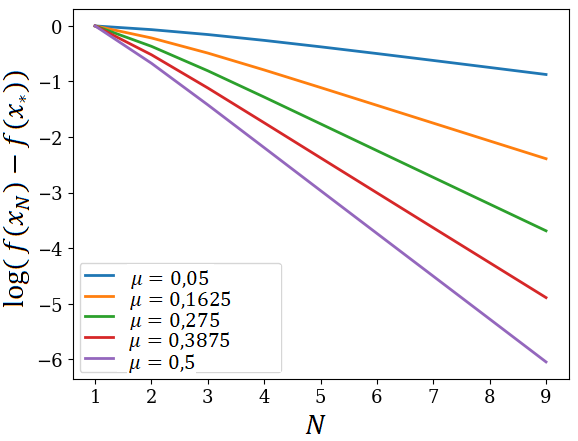
\includegraphics[width=\textwidth]{linear_convergence.png}
         \caption{График зависимости невязки $(f(x_N) - f_{\star})$ от номера итерации $N$ при $\varepsilon = 0.5$. Демонстрирует линейную сходимость.}
         \label{fig:linear_conv}
     \end{subfigure}
     \hfill
     \begin{subfigure}[b]{0.45\textwidth}
         \centering
         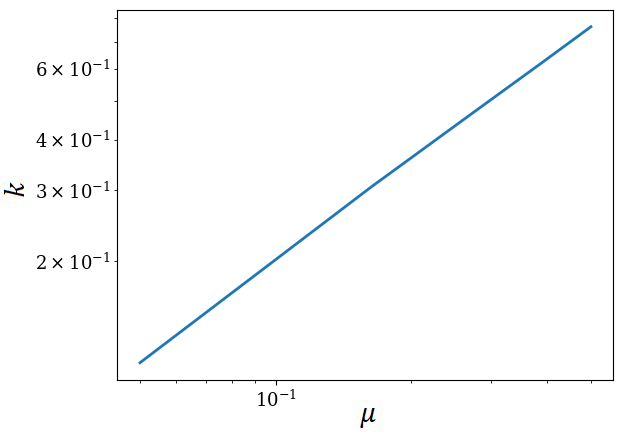
\includegraphics[width=\textwidth]{q_mu_grqph.png}
         \caption{График зависимости график $k(\mu)$ при $\varepsilon = 0.5$. Демонстрирует зависимость скорости сходимости только лишь от $\left(\frac{\mu}{L}\right)^{\alpha(\varepsilon)}$.}
         \label{fig:three sin x}
     \end{subfigure}
     \hfill
        \caption{Вычислительные эксперименты}
        \label{fig:two graphs}
\end{figure}


Повторим эксперимент для различных $\varepsilon$ и построим график $\alpha(\varepsilon)$ (\ref{fig:main_res}).
\begin{figure}[htp]
\centering
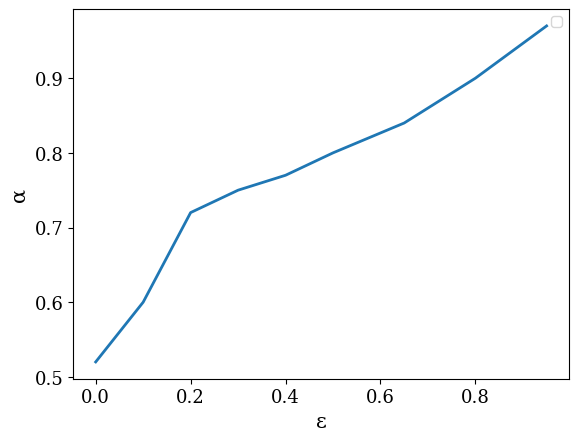
\includegraphics[width=0.5\textwidth]{main_res__of_gfom.png}
    \caption{График зависимости $\alpha(\varepsilon)$.}
    \label{fig:main_res}
\end{figure}

\subsection{Результаты и их обсуждение}

Результаты вычислительных экспериментов не противоречат гипотезе. Скорость сходимости метода NoisyGFOM зависит от шума $\varepsilon$. При увеличении шума скорость сходимости падает от быстрой \eqref{GFOMconverge} до свойственной обычному градиентному спуску \eqref{GDconverge}. Итак, 
\begin{equation}\label{NoisyGFOMconverge}
   f(x_N) - f_{\star} = O\left(\left(\frac{1 - \left(\frac{\mu}{L}\right)^{\alpha(\varepsilon)}}{1 + \left(\frac{\mu}{L}\right)^{\alpha(\varepsilon)}}\right)^N\right),  \
   \alpha|_{\varepsilon = 0} = \frac12, \ \alpha|_{\varepsilon = 1} = 1
\end{equation}

\section{Заключение}
В данной работе было исследовано влияние зашумленного градиента \eqref{inexact_grad} на жадный метод оптимизации первого порядка NoisyGFOM. Так, при появлении шума в градиентах метод сохраняет свою линейную сходимость при $\varepsilon \in [0,1]$, уменьшая скорость сходимости с увеличением шума. При шуме $\varepsilon \approx 1$ скорость сходимости NoisyGFOM совпадает со скоростью сходимости градиентного спуска \eqref{GDconverge}, а при $\varepsilon \approx 0$ - со скоростью сходимости ускоренных методов \eqref{GFOMconverge}.
В наши дальнейшие планы входит теоретическое обоснование полученных экспериментально результатов.



\begin{comment}
\section{Вычислительный эксперимент}
Для алгоритма ISTM в статье \cite{kornilov2023intermediate} была доказана следующая теорема.

\begin{theorem}\label{theo:coveregence_alg1}
Пусть функция $f$ -- выпуклая и $L$-гладкая с относительным шумом $\hat{\varepsilon} \in [0,1]$. Тогда после $N\geq 1$ итераций алгоритма  \texttt{ISTM} с промежуточным параметром $p \in [1,2]$ и 
\begin{equation}\label{formula_for_a}
    a = C \cdot \max{\{1, N^p \hat{\varepsilon}^2\}},\ C = 2304
\end{equation}
имеем невязку на $N$-ой итерации, равную 
\begin{equation}\label{conv_rate_alg1}
    f(y^N) - f(x^*) \leq \frac{8 a L R_0^2}{(N+1)^p},
\end{equation}
где $R_0 = \|x^0 - x^*\|_2$ 
или, если подставить параметр $a$ из \eqref{formula_for_a}, имеем
\begin{equation}\label{eq:conv_rate_alg1_proper_a}
f(y^N) - f(x^*) \leq 8C \cdot \max \left\{ \frac{LR_0^2}{N^p}, \hat{\varepsilon}^2 L R_0^2 \right\}.
\end{equation}
\end{theorem}

Теорема говорит о том, что при номерах итераций $N$ таких, что $N^p \hat{\varepsilon}^2 \le 1$, алгоритм сходится со скоростью $\sim \frac{1}{N^p}$. При больших номерах итераций, из-за наличия относительной погрешности в определении градиента, алгоритм выходит на вынужденное плато по невязке, равное $f(y^N) - f(x^*) = 8C \cdot \hat{\varepsilon}^2 L R_0^2$. Далее мы будем рассматривать случай $p = 2$ в силу его наиболее быстрой сходимости.

В этой теореме смущает довольно большая константа $C = 2304$. Однако она была получена авторами теоремы с применением не самых жестких неравенств. Численные эксперименты с применением техники PEP демонстрируют, что фактически эта константа значительно меньше. Цель нашего вычислительного эксперимента --- уточнить эту константу.

Для этого мы решим следующую задачу оптимизации с фиксированными  $N, \hat{\varepsilon}$ и $a$.

\begin{equation}\label{eq:max_problem_intro}
 \tau^N := \max\limits_{n, f, x^0} f(x^N) - f(x^*),   
\end{equation}
с условиями выпуклости и $L$-гладкости функции $f:\R^n \rightarrow \R$ , $0 \in \nabla f(x^*)$ и 
\begin{eqnarray} 
    && \|x^0 - x^*\|^2_2 \leq R^2,  \\
    && \|\widetilde{\nabla} f(x^k) - \nabla f(x^k)\|^2_2 \leq \hat{\varepsilon}^2 \|\nabla f(x^k)\|^2_2, \quad k = \overline{0,  N-1}, \label{eq:pep_rel} \\
    && x^{k+1}, y^{k+1}, z^{k+1} = \text{ISTMstep}(x^{k}, y^k, z^k, \widetilde{\nabla} f(x^k)), \quad k = \overline{0,  N-1}.\label{eq:pep_istm}
\end{eqnarray}

Таким образом, мы ищем функцию $f$ из класса $\mathcal{F}_{0, L}$, дающую на $N$-ой итерации алгоритма \texttt{ISTM} с относительным шумом $\hat{\varepsilon}$ наибольшее значение невязки $\tau^N$. Как уже ранее в этой статье обсуждалось, такая задача может быть переформулирована в конечномерную задачу полуопределенного программирования (техника PEP) и решена численно с помощью специальных решателей. Мы будем использовать MOSEK solver \cite{aps2019mosek} и PEPit framework \cite{goujaud2022pepit}.

\subsection{Качественная демонстрация сходимости}

С помощью решателей исследовалась задача \eqref{eq:max_problem_intro} для $p = 2$. Было показано, что теоретическое плато по невязке действительно достигается. Плато тем больше, чем больше шум.

\begin{figure}[htp]
\centering
{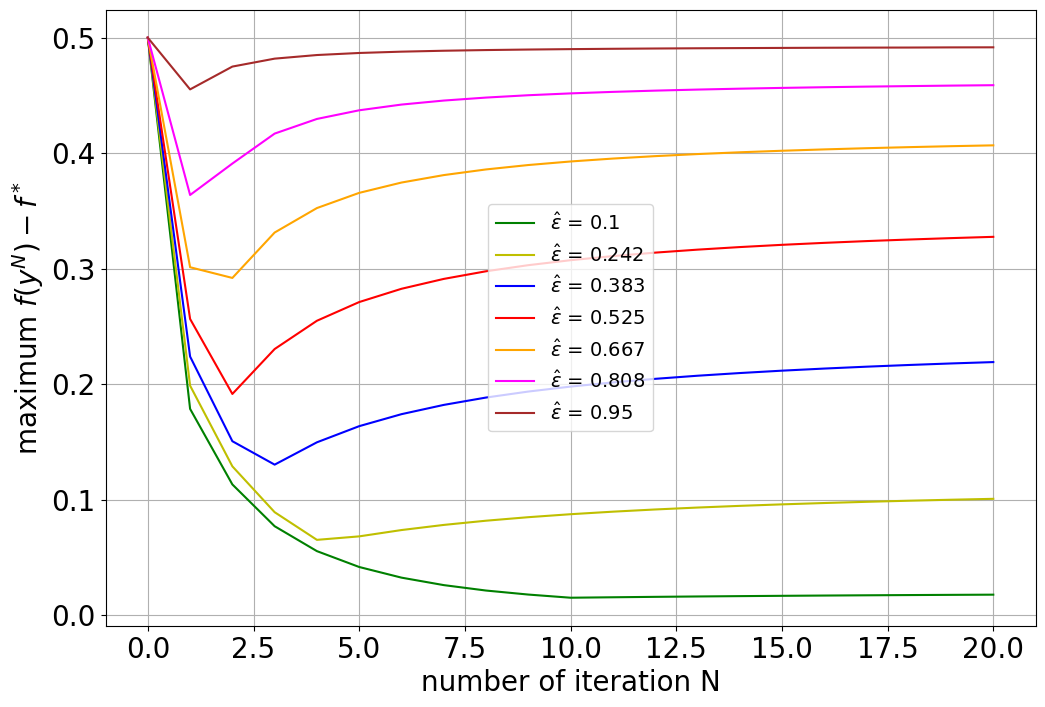
\includegraphics[width=10cm]{convergence_rate.png} }
\caption{Графики зависимостей максимальной невязки $\tau^N$ в зависимости от номера итерации $N$ алгоритма \texttt{ISTM} для различных значений шумов $\hat{\varepsilon}$ и при фиксированных $p = 2, L = 1, R = 1$. }
\label{fig:conv_with_opt_a_diff_p}
\end{figure}

\subsection{Уточнение константы $C$ из теоремы \ref{theo:coveregence_alg1}}

Согласно теореме \ref{theo:coveregence_alg1}, алгоритм \texttt{ISTM} перестает монотонно убывать на итерации $N_{theory} (a,\hat{\varepsilon}, p) = (\frac{a}{C \hat{\varepsilon}^2})^{\frac{1}{p}}$. Проведем численный эксперимент, который при фиксированном $p = 2$ и для разных параметров $a$ будет искать номер $N_{pep}$, при котором последовательность невязок $\{\tau^N\}$, полученных из \eqref{eq:max_problem_intro}, перестает убывать. Построим график $N_{pep}^2 \hat{\varepsilon}^2 (a) = \frac{1}{C} a$. Его линейность будет подтвержать теоретический характер зависимости из \ref{theo:coveregence_alg1}, а угловой коэффициент позволит уточнить (уменьшить) константу $C$.

\begin{figure}[htp]
\centering
{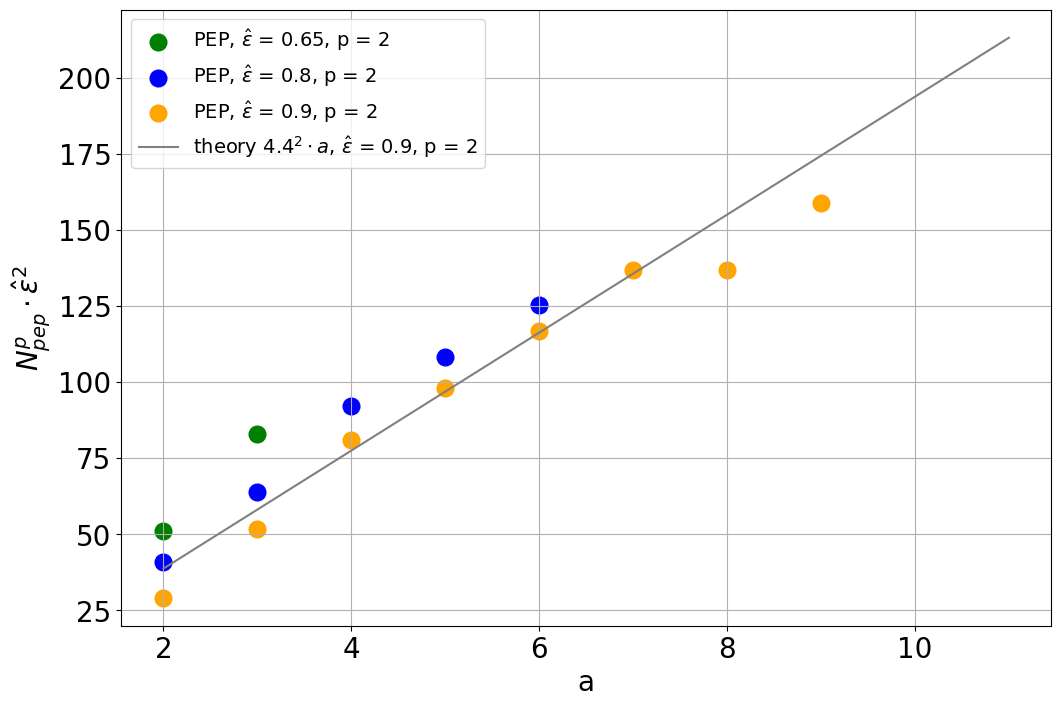
\includegraphics[width=10cm]{find_c.png} }
\caption{Графики зависимости номера итерации $N_{pep}$, при которой начинается расходимость метода \texttt{ISTM}, в зависимости от параметра $a$ для разных значений шума $\hat{\varepsilon}$. Для наглядного подтверждения теории, график построен в координатах $N_{pep}^2 \hat{\varepsilon}^2 (a)$, в которых график становится линейным. Параметры $p = 2, L = 1, R = 1$. }
\label{fig:conv_with_opt_a_diff_p}
\end{figure}

Параметры прямой линии, проходящей через точки, были определены с помощью линейной регрессии (метода наименьших квадратов). Полученный результат $C \approx \frac{1}{4.4^2}$ существенно меньше завышенной теоретической константы $C = 2304$.
\end{comment}






\bibliographystyle{unsrtnat}
\bibliography{references}

\end{document}







\bibliographystyle{unsrtnat}
\bibliography{references}

\end{document}
